\documentclass{report}

\usepackage{tikz}
 \usetikzlibrary{shapes,arrows} 
 
 % Define block styles
 \tikzstyle{decision} = [diamond, draw, fill=blue!20, text width=4.5em, text badly centered, node distance=3cm, inner sep=0pt]
 \tikzstyle{data} = [draw, rectangle, fill=red!20, node distance=3cm, text centered, text width=6em, rounded corners, minimum height=3em]
 \tikzstyle{line} = [draw, -latex']
 \tikzstyle{computing} = [rectangle, draw, fill=blue!20, text width=5em, text centered, minimum height=4em] 

 \pgfdeclarelayer{background}
 \pgfdeclarelayer{foreground}
 \pgfsetlayers{background,main,foreground}
%----------------------

\title{Analysis and Design Document \\ for \\ OPAL}
\begin{document}
\maketitle
\chapter{Introduction}

\par The primary goal is create a framework that helps the users to realize the tunning task following the schema


\begin{figure}[htpb]
  \centering
  
  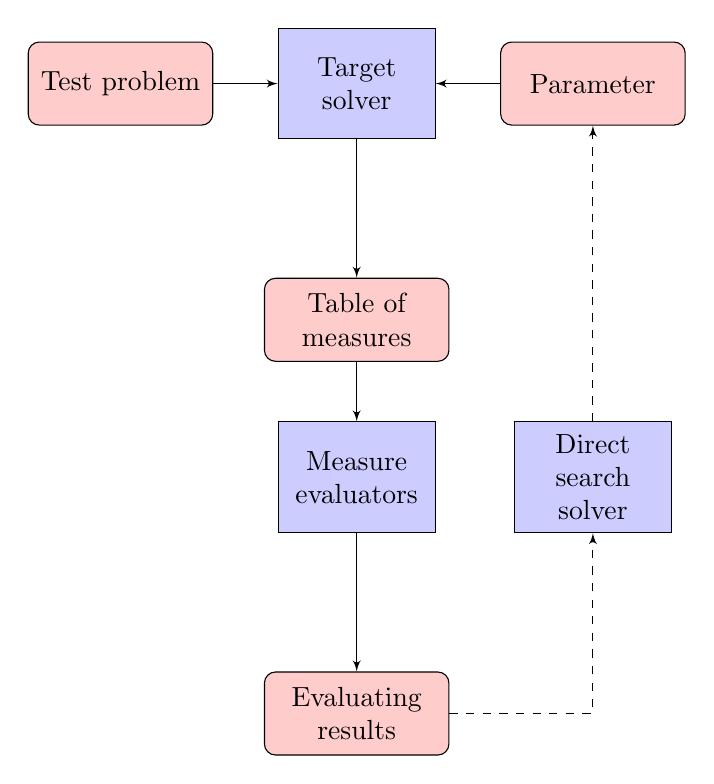
\begin{tikzpicture}[node distance = 2cm, auto]
    % Place nodes
    \node [computing] (algorithm) {Target solver};
    \node [data,left of=algorithm] (test-prob) {Test problem};
    \node [data, right of=algorithm] (param) {Parameter};
    \node [data, below of=algorithm] (measure-table) {Table of measures};
    \node [computing, below of=measure-table] (evaluator) {Measure evaluators};
    %\node [data, left of=evaluator, node distance=3.5cm] (model) {Evaluating model};
    \node [data, below of=evaluator] (evaluating-results) {Evaluating results};
    \node [computing, right of=evaluator, node distance=3cm] (solver) {Direct search solver};
    % Draw edges
    \path [line] (test-prob) -- (algorithm);
    \path [line] (param) -- (algorithm);
    \path [line] (algorithm) -- (measure-table);
    \path [line] (measure-table) -- (evaluator);
    %\path [line] (model) -- (evaluator);
    \path [line] (evaluator) -- (evaluating-results);
    \path [line,dashed] (evaluating-results) -| (solver);
    \path [line,dashed] (solver) -- (param);
\end{tikzpicture}
  \caption{General schema of parameter tunning}
  \label{fig:parameter-tunning-schema}
\end{figure}
\chapter{Backgrounds}
\par The principles are built basing on the observations:
\begin{itemize}
  \item There are main entities Information and Information Manipulator
    \begin{enumerate}
    \item Information is in fact set of elements with the methods set and get value. The 
      set is organized in the different structure like a scalar, a vector or a matrix ...
    \item Information Manipulator represent for the processes manipulate the input information to
      get the other information as output
    \end{enumerate}
  \item Other the set and get methods for each element, the Information may be combined by the 
    set operation like union, extract, subset v�rification.
  \item An Information Manipulator is characterized by Input, Parameters and Output.
    \begin{enumerate}
    \item Input includes the Information and set of Manipulators that may 
      be a empty set. If this set is empty, the Manipulator is called Evaluator, otherwise
      it is called Solver. 
    \item Parameter is actually Information, it is used to generallized a class of Manipulator.
      Each time the parameters are set to the specific values, we have a manipulator.
    \item Output is Information represents for the results of manipulation.
    \end{enumerate}
  \item Any process is formulated by the combinations of the manipulators
    \begin{enumerate}
      \item Sequence of evaluator: Output of the first evaluator is input of the second evaluator
      \item Support: A solver may be used the other evaluator during processing Information
      \item Cooperation: Two manipulator have the same Input.
    \end{enumerate}
  \item The relations amongs Manipulators are:
    \begin{enumerate}
    \item Dependence: A manipulator depends on the others if it used the others to proccess 
      the Information
      \item Composite: A manipulator can be decomposed as combinations of the others
    \end{enumerate}
  \end{itemize}

\chapter{System analysis}
We apply the principle above to describe the framework in a typical use-case.
\begin{figure}[htpb]
  \centering
  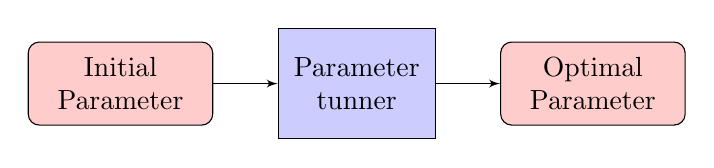
\begin{tikzpicture}[node distance = 2cm, auto]
    % Place nodes
    \node [computing] (tunner) {Parameter tunner};
    \node [data,left of=tunner] (initial-param) {Initial Parameter};
    \node [data, right of=tunner] (optimal-param) {Optimal Parameter};
    % Draw edges
    \path [line] (initial-param) -- (tunner);
    \path [line] (tunner) -- (optimal-param);
\end{tikzpicture}
  \caption{Top view of tunning parameter}
  \label{fig:top-view}
\end{figure}

\begin{figure}[htpb]
   % We need layers to draw the block diagram
  \centering
  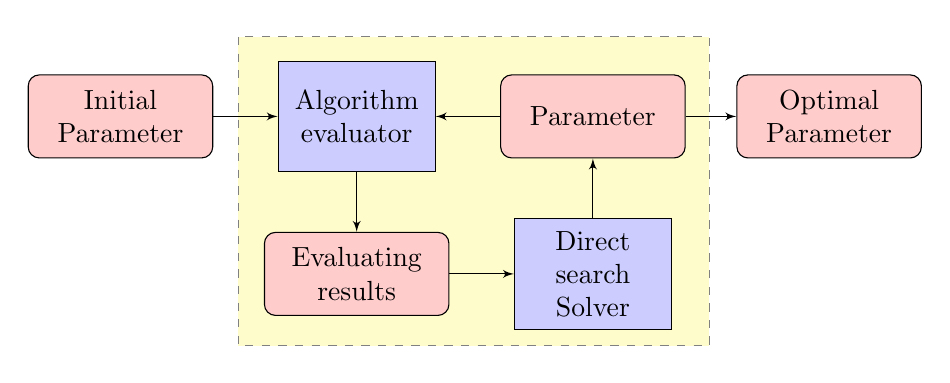
\begin{tikzpicture}[node distance = 2cm, auto]
   
    % Place nodes
    \node [computing] (evaluator) {Algorithm evaluator};
    \node [data,left of=evaluator] (initial-param) {Initial Parameter};
    \node [data, below of=evaluator, node distance = 2cm] (eval-result) {Evaluating results};
    \node [data, right of=evaluator] (param) { Parameter};
    \node [data, right of=param] (optimal-param) {Optimal Parameter};
    \node [computing, below of=param] (solver) {Direct search Solver};
    % Draw edges
    \path [line] (initial-param) -- (evaluator);
    \path [line] (evaluator) -- (eval-result);
    \path [line] (eval-result) -- (solver);
    \path [line] (solver) -- (param);
    \path [line] (param) -- (evaluator);
    \path [line] (param) -- (optimal-param);
    % Now it's time to draw the colored tunner rectangles.
    % To draw them behind the blocks we use pgf layers. This way we  
    % can use the above block coordinates to place the backgrounds   
    \begin{pgfonlayer}{background}
        % Compute a few helper coordinates
        \path (evaluator.west |- evaluator.north)+(-0.5,0.3) node (a) {};
        \path (solver.south -| param.east)+(+0.3,-0.2) node (b) {};
        \path[fill=yellow!20, draw=black!50, dashed]
            (a) rectangle (b);
    \end{pgfonlayer}
\end{tikzpicture}
  \caption{Black box optimization view of tunning parameter}
  \label{fig:blackbox-view}
\end{figure}

\begin{figure}[htpb]
   % We need layers to draw the block diagram
  \centering
  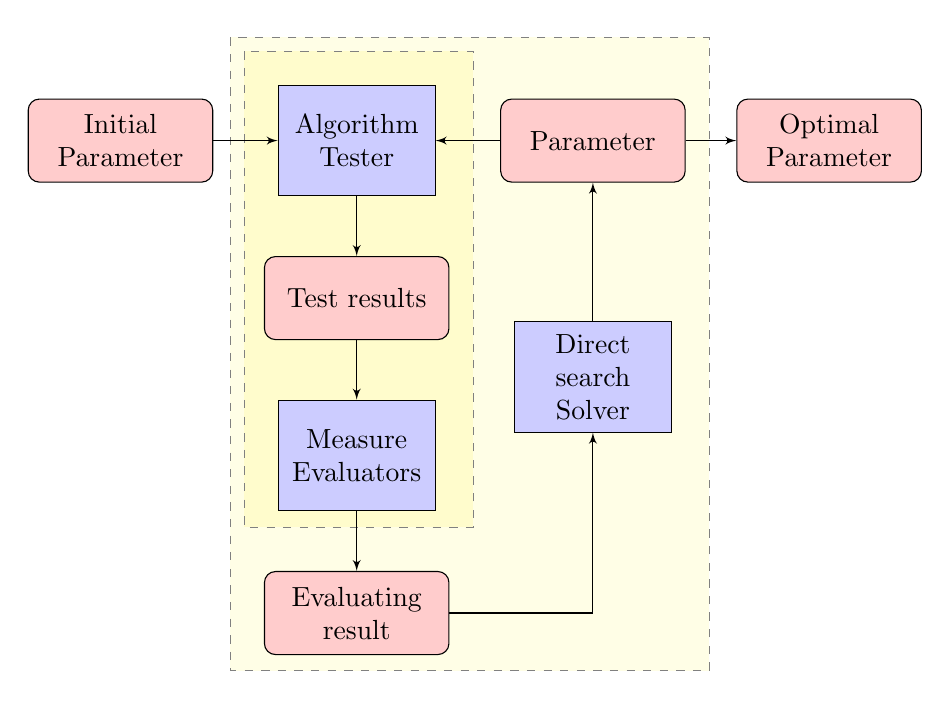
\begin{tikzpicture}[node distance = 2cm, auto]
   
    % Place nodes
    \node [computing] (algo-tester) {Algorithm Tester};
    \node [data,left of=algo-tester] (initial-param) {Initial Parameter};
    \node [data, below of=algo-tester,node distance = 2cm] (test-result) {Test results};
    \node [computing, below of=test-result] (evaluators) {Measure Evaluators};
    \node [data, below of=evaluators, node distance = 2cm] (eval-result) {Evaluating result};
    \node [data, right of=algo-tester] (param) { Parameter};
    \node [data, right of=param] (optimal-param) {Optimal Parameter};
    \node [computing, below of=param, node distance = 3cm] (solver) {Direct search Solver};
    
    % Draw edges
    \path [line] (initial-param) -- (algo-tester);
    \path [line] (algo-tester) -- (test-result);
    \path [line] (test-result) -- (evaluators);
    \path [line] (evaluators) -- (eval-result);
    \path [line] (eval-result) -| (solver);
    \path [line] (solver) -- (param);
    \path [line] (param) -- (algo-tester);
    \path [line] (param) -- (optimal-param);
    % Now it's time to draw the colored tunner rectangles.
    % To draw them behind the blocks we use pgf layers. This way we  
    % can use the above block coordinates to place the backgrounds   
    \begin{pgfonlayer}{background}
       % Compute a few helper coordinates
      \path (algo-tester.west |- algo-tester.north)+(-0.6,0.6) node (a) {};
      \path (eval-result.south -| param.east)+(+0.3,-0.2) node (b) {};
      \path[fill=yellow!10, draw=black!50, dashed]
      (a) rectangle (b);
      % Compute a few helper coordinates
      \path (a.west |- a.north)+(+0.3,-0.3) node (c) {};
      \path (evaluators.south -| test-result.east)+(+0.3,-0.2) node (b) {};
      \path[fill=yellow!20, draw=black!50, dashed]
      (c) rectangle (b);
     
    \end{pgfonlayer}
\end{tikzpicture}
  \caption{Empirical test view of tunning parameter}
  \label{fig:test-view}
\end{figure}

\begin{figure}[hpbt]
  \centering
  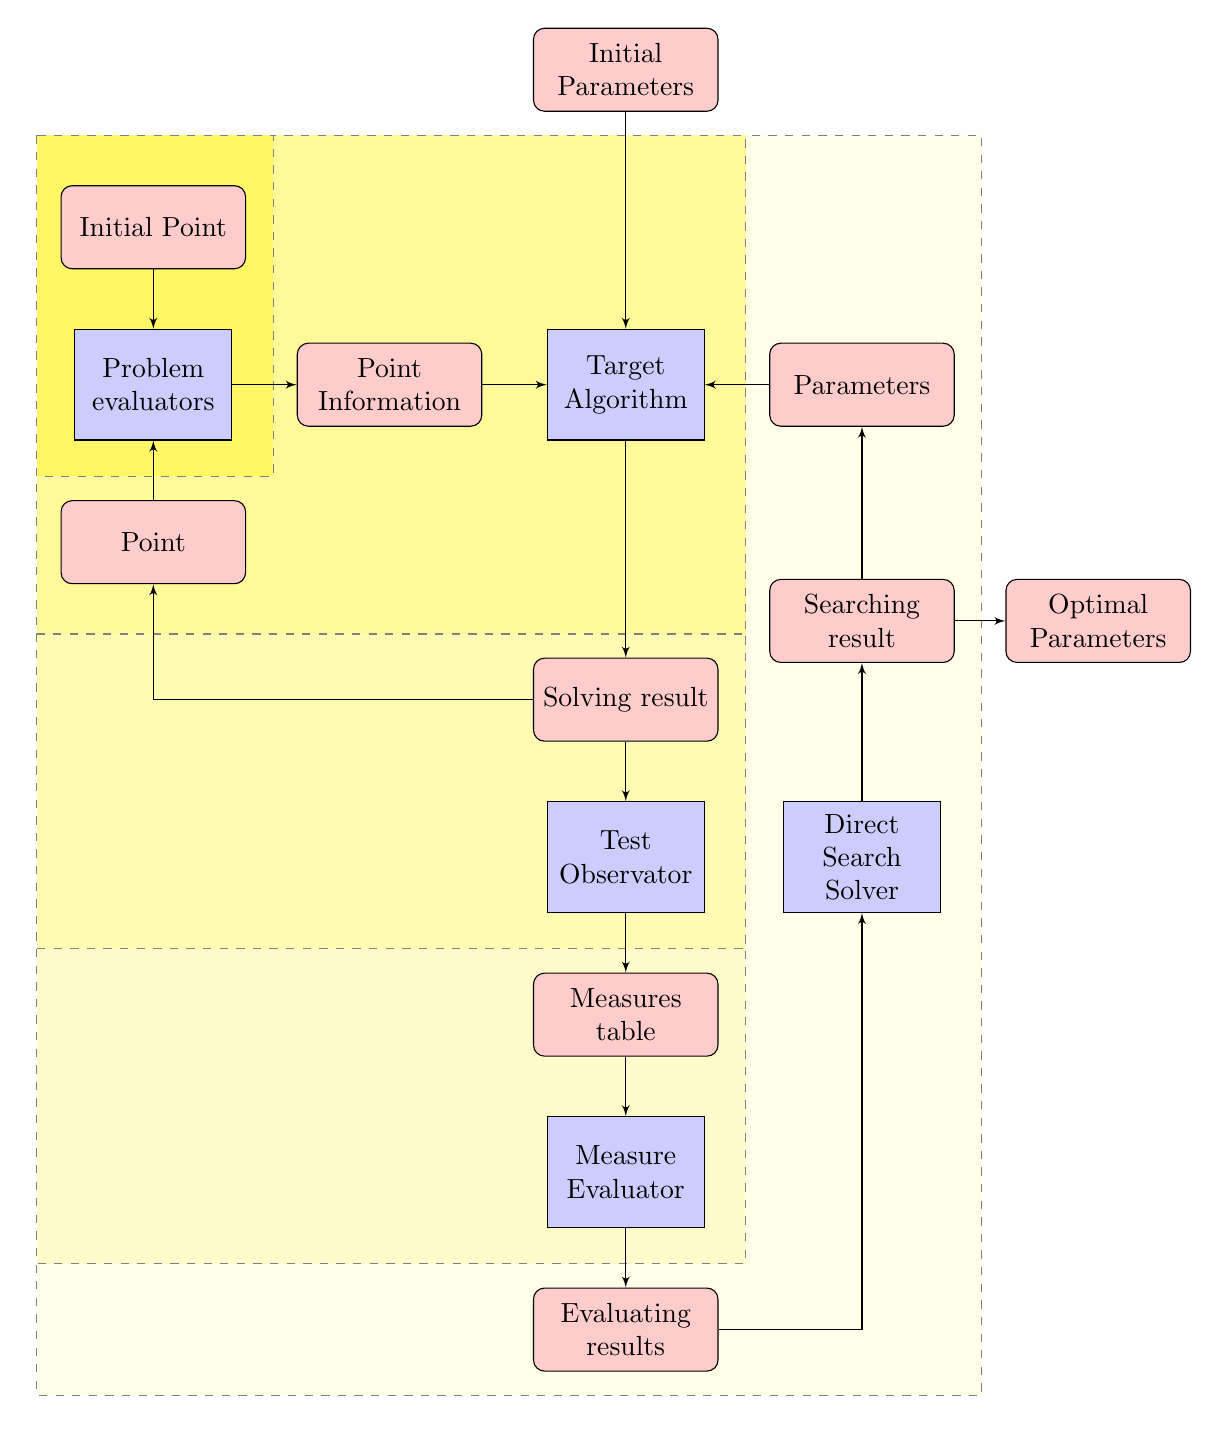
\begin{tikzpicture}[node distance=2cm, auto]
    \node [data] (initial-point){Initial Point};
    \node [computing, below of=initial-point](evaluator){Problem evaluators};
    \node [data, right of=evaluator, node distance=3cm](info){Point Information};
    \node [data, below of=evaluator, node distance=2cm](point){Point};
    \node [computing, right of=info, node distance=3cm](algorithm){Target Algorithm};
    \node [data, right of=algorithm](param){Parameters};
    \node [data, above of=algorithm, node distance= 4cm](initial-param){Initial Parameters};
    \node [data, below of=algorithm, node distance=4cm](solv-result){Solving result};
    \node [computing, below of=solv-result](test-observator){Test Observator};
    \node [data, below of=test-observator, node distance=2cm](measure-table){Measures table};
    \node [computing, below of=measure-table](measure-evaluators){Measure Evaluator};
    \node [data, below of=measure-evaluators, node distance=2cm](eval-result){Evaluating results};
    \node [data, below of=param](ds-solv-result){Searching result};
    \node [computing, below of=ds-solv-result,node distance=3cm](ds-solver){Direct Search Solver};
    \node [data, right of=ds-solv-result](opt-param){Optimal Parameters};

    \path [line](initial-point) -- (evaluator);
    \path [line](evaluator) -- (info);
    \path [line](info) -- (algorithm);
    \path [line](algorithm) -- (solv-result);
    \path [line](solv-result) -| (point);
    \path [line](point) -- (evaluator);
    \path [line](solv-result) -- (test-observator);
    \path [line](test-observator) -- (measure-table);
    \path [line](measure-table) -- (measure-evaluators); 
    \path [line](measure-evaluators) -- (eval-result);
    \path [line](eval-result) -| (ds-solver);
    \path [line](ds-solver) -- (ds-solv-result);
    \path [line](ds-solv-result) -- (param);
    \path [line](param) -- (algorithm);
    \path [line](initial-param) -- (algorithm);
    \path [line](ds-solv-result) -- (opt-param);
    \begin{pgfonlayer}{background}
       \path (initial-point.west |- initial-param.south)+(-0.3,-0.3) node (a) {};
       \path (opt-param.west |- eval-result.south)+(-0.3,-0.3) node (b) {};
       \path[fill=yellow!10, draw=black!50, dashed]
       (a) rectangle (b);
       
       \path (eval-result.north -| param.west)+(-0.3,0.3) node (b) {};
       \path[fill=yellow!20, draw=black!50, dashed]
       (a) rectangle (b);

       \path (measure-table.north -| param.west)+(-0.3,0.3) node (b) {};
       \path[fill=yellow!30, draw=black!50, dashed]
       (a) rectangle (b);
       
       \path (solv-result.north -| param.west)+(-0.3,0.3) node (b) {};
       \path[fill=yellow!40, draw=black!50, dashed]
       (a) rectangle (b);

       \path (point.north -| info.west)+(-0.3,0.3) node (b) {};
       \path[fill=yellow!60, draw=black!50, dashed]
       (a) rectangle (b);
    \end{pgfonlayer}
  \end{tikzpicture}
  \caption{Algorithm view}
  \label{fig:algorithm-view}
\end{figure}
\chapter{System design}

\end{document}